$subject$=Математическая статистика
$teacher$=Лекции Блаженова А. В.
$date$=08.04.2025

\section{Лекция 9.}

\subsection{Исследование статистической корреляции}

\subsubsection{Математическая модель регрессии}

Пусть случайная величина $X$ зависит от случайной величины $Z$ (необязательно случайной)

\Def Регрессией $X$ на $Z$ называется функция $f(z) = E(X|Z = z)$. 
Она показывает зависимость среднего значения $X$ от значения $Z$

Уравнение $x = f(z)$ называется уравнением регрессии, а график этой функции - линия регрессии

Пусть при $n$ экспериментах при значениях $Z_1, Z_2, \dots, Z_n$ фактора $Z$ наблюдались значения
$X_1, X_2, \dots, X_n$ случайной величины $X$

Обозначим через $\varepsilon_i$ разницу между экспериментальным и теоретическими значениями случайной величины $X$,
то есть $\varepsilon_i = X_i - f(z_i)$

$\varepsilon$ - это случайный член модели или так называемая теоретическая ошибка

\Nota Обычно можно считать, что $\varepsilon_i$ независимы друг от друга и имеет нормальное распределение с $a = 0$,
так как $E\varepsilon_i = E(X_i - f(Z_i)) = E(X | Z = Z_i) - E(X | Z = Z_i) = 0$

Цель: нам нужно по экспериментальным данным $(z_1, x_1), \dots, (z_n, x_n)$ как можно лучше оценить функцию $f(z)$

\Notas При этом предполагая (часто из теории), что $f(z)$ - функция определенного вида, но параметры которой неизвестны.
Если нет, то начинаем подбирать модели самого простого вида. В противном случае, наилучшим решением была бы кривая, 
проходящая через все точки 

\subsubsection{Метод наименьших квадратов}

Пусть известен из теории вид функции $f(z)$. Метод наименьших квадратов состоит в выборе параметров $f(z)$ таким образом,
чтобы минимизировать сумму квадратов ошибок $\sum_{i = 1}^n \varepsilon_i^2 = \sum_{i = 1}^n (X_i - f(Z_i))^2 \rightarrow \min$

\Def Пусть $\theta$ - набор неизвестных параметров функции $f(z)$. Оценка $\hat \theta$ параметра $\theta$, 
при которой достигается минимум $\sum_{i = 1}^n \varepsilon_i^2$, называется оценкой метода наименьших квадратов (или ОМНК)

\subsubsection{Линейная парная регрессия}

Пусть имеется теоретическая модель линейной регрессии 

$f(z) = \alpha + \beta z + \varepsilon$ - теоретическая модель, где $\varepsilon$ - теоретическая ошибка
отражающая влияние невключенных в модель факторов, возможной нелинейности, ошибок измерения и просто случая

Пусть $(z_1, x_1), \dots, (z_n, x_n)$ - экспериментальные данные. По ним методом наименьших квадратов строим
экспериментальную модель линейной регрессии $f(z) = a + b z$, где $a$ и $b$ - ОМНК параметров $\alpha$ и $\beta$

$\hat \varepsilon_i = X_i - f(Z_i) = X_i - (a + b Z_i)$ - экспериментальная ошибка

Найдем ОМНК параметров $\alpha$ и $\beta$

$\sum_{i = 1}^n \hat \varepsilon_i^2 = \sum_{i = 1}^n (X_i - (a + b Z_i))$

$\frac{\partial}{\partial a} \sum_{i = 1}^n \hat \varepsilon_i^2 = \sum_{i = 1}^n -2 (X_i - a - b Z_i) = 
-2 \sum_{i = 1}^n X_i + 2\sum_{i = 1}^n a + 2b \sum_{i = 1}^n Z_i = -2(n \overline{x} - na - bn \overline{z})$

$\frac{\partial}{\partial b} \sum_{i = 1}^n \hat \varepsilon_i^2 = \sum_{i = 1}^n -2 Z_i (X_i - a - b Z_i) = 
-2 \sum_{i = 1}^n X_i Z_i + 2\sum_{i = 1}^n a Z_i + 2b \sum_{i = 1}^n Z_i^2 = -2(n \overline{x z} - a n \overline{z} - bn \overline{z^2})$

\begin{cases}
    -2 (n \overline{x} - na - nb \overline{z}) = 0 \\
    -2 (n \overline{zx} - na \overline{z} - nb \overline{z^2}) = 0 \\
\end{cases} $\Longleftrightarrow$ \begin{cases}
    a + b\overline{z} = \overline{x} \\
    a\overline{z} + b \overline{z^2} = \overline{zx} \\
\end{cases} 

Получили систему линейных уравнений. Будем называть ее нормальной системой. При решении получаем:

\begin{cases}
    a = \overline{x} - b \overline{z} \\
    (\overline{x} b \overline{z}) \overline{z} + b \overline{z^2} = \overline{zx} \\
\end{cases} $\Longleftrightarrow$ \begin{cases}
    a = \overline{x} - b \overline{z} \\
    b = \frac{\overline{zx} - \overline{z} \, \overline{x}}{\hat \sigma^2_z}
\end{cases} - ОМНК 

Запишем уравнение линейной регрессии в удобном виде: $\overline{x}_z = f(z) = E(X | Z = z)$

$\overline{x}_z = a + bz$

$\overline{x}_z = \overline{x} - b \overline{z} + bz$

$\overline{x}_z - \overline{x} = \frac{\overline{z x} - \overline{x} \, \overline{z}}{\hat \sigma^2_z} (z - \overline{z})$

$\overline{x}_z - \overline{x} = \frac{\hat \sigma_x}{\hat \sigma_z} \frac{\overline{z x} - \overline{x} \, \overline{z}}{\hat \sigma_z \hat \sigma_x} (z - \overline{z}) = 
\frac{\hat \sigma_x}{\hat \sigma_z} \hat r (z - \overline{z})$, где $\hat r$ - выборочный коэффициент линейной корреляции

Или $\frac{\overline{x}_z - \overline{x}}{\hat \sigma_x} = \hat r \frac{z - \overline{z}}{\hat \sigma_z}$ - выборочное уравнение линейной регрессии

\Nota Прямая регрессии проходит через точку из выборочных средних

\Notas При $n \to \infty$ $\overline{x} \longrightarrow EX, \overline{z} \longrightarrow EZ, \hat \sigma_x \longrightarrow \sigma_x,
\hat \sigma_z \longrightarrow \sigma_z, \overline{x}_z \longrightarrow E(X | Z = z), \hat r \longrightarrow r$, получаем 
$\frac{E(X | Z = z) - EX}{\sigma_x} = r \frac{z - EZ}{\sigma_z}$ - теоретическое уравнение линейной регрессии

\subsubsection{Геометрический смысл линии регрессии}

% https://www.geogebra.org/calculator/pvvdv7ch

\begin{center}
    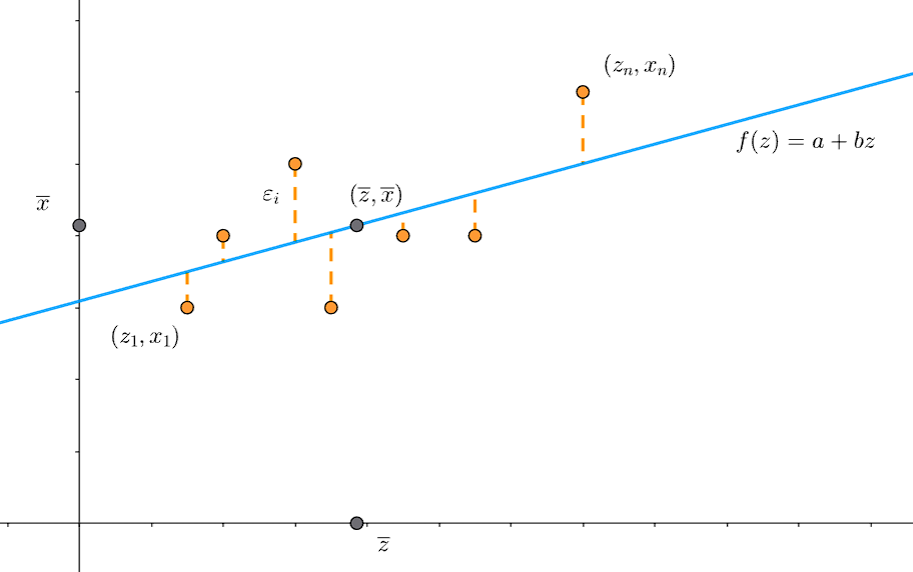
\includegraphics[height=9cm]{mathstat/images/mathstat_2025_04_08_1}
\end{center}

Суть МНК: находим такую прямую, чтобы сумма квадратов длин этих отрезков (по сути отклонений) была минимальна 
(или дисперсия экспериментальных данных относительно прямой была минимальна)


\subsubsection{Выборочный коэффициент линейной корреляции}

\Def $\hat r = \frac{\overline{z x} - \overline{x} \, \overline{z}}{\hat \sigma_z \hat \sigma_x}$ называется выборочным коэффициентов 
линейной корреляции. Ясно, что она будет точечной оценкой теоретического коэффициента линейной корреляции. 
Также $\hat r$ является несмещенной оценкой

Поэтому выборочный коэффициент корреляции характеризует силу линейной связи. Знак коэффициента показывает направления корреляции (прямая или обратная)

Силу связи можно примерно оценить от шкале Чеддока:

\smallvspace

\begin{tabular}{c|l}
    Количественная мера $\hat r$ & Качественная мера \\
    \hline
    $0.1 \ \textendash \ 0.3$ & Слабая \\
    $0.3 \ \textendash \ 0.5$ & Умеренная \\
    $0.5 \ \textendash \ 0.7$ & Заметная \\
    $0.7 \ \textendash \ 0.9$ & Высокая \\
    $> 0.9$ & Весьма высокая \\
\end{tabular}

\mediumvspace

\subsection{Проверка гипотезы о значимости выборочного коэффициента корреляции}

Пусть $(Z, X)$ распределена нормально. По выборке объема $n$ вычислен выборочный коэффициент корреляции $\hat r$, а $r$ - теоретический коэффициент корреляции

Проверяется $H_0 : r = 0$ (выборочный коэффициент корреляции статистически незначим) против $H_1 : r \neq 0$ (коэффициент статистически значим)

\begin{MyTheorem}
    Если $H_0$ верна, то $K = \frac{\hat r \sqrt{n - 2}}{\sqrt{n - \hat r^2}} \in T_{n - 2}$ - распределение Стьюдента с степенью $n - 2$ 
\end{MyTheorem}

Получаем критерий. Пусть $t_\alpha$ - квантиль $|T_{n - 2}|$ (двухстороннее распределение Стьюдента) уровня $\alpha$

\begin{cases}
    H_0 : r = 0, & \text{ если } |K| < t_\alpha \\
    H_1 : r \neq 0, & \text{ если } |K| \geq t_\alpha \\
\end{cases}

Надо понимать, что корреляция - более тонкое понятие, чем зависимость

А термин \textit{регрессия} получил свое название чисто исторически: статистик Гальтон в 1886 году 
исследовал зависимость роста детей от роста родителей

$E(\text{Р}_\text{сына} | Z_\text{отца} = Z_1, Z_\text{матери} = Z_1) = 0.27 Z_1 + 0.2 Z_2 + \operatorname{const}$

$E(\text{Р}_\text{дочери} | Z_\text{отца} = Z_1, Z_\text{матери} = Z_1) = \frac{1}{1.08} \text{Р}_\text{сына}$

Дальше он заметил, что при у самых высоких родителей рост детей был меньше относительно них (скатывался к среднему, происходил регресс)

Позже исследовали экономические результаты фирм, показатели спортсменов, которые после успешного сезона уменьшались, 
после чего появлялось куча теорий. Сейчас все это объясняется простым случаем

\subsection{Выборочное корреляционное отношение}

Выборочный коэффициент корреляции характеризует только силу линейной связи. Следующий подход основан на однофакторном дисперсионном анализе

Пусть есть $k$ выборок случайной величины $X$ при $k$ различных уровнях фактора $Z$. Вычислены общая, внутригрупповая и межгрупповая дисперсии. 
По теореме $D_\text{О} = D_\text{М} + D_\text{В}$

\Def Выборочным корреляционным отношением $X$ на $Z$ называется величина $\eta_{X, Z} = \sqrt{\frac{D_\text{М}}{D_\text{О}}}$

\underline{Свойства}:

\begin{enumerate}
    \item $0 \leq \eta_{X, Z} \leq 1$ ($D_\text{М}, D_\text{О} \geq 0$)

    \item Если $\eta = 1$, то $D_\text{М} = D_\text{О} \Longrightarrow D_\text{В} = 0$, имеем функциональную зависимость $X$ от $Z$

    \item Если $\eta = 0$, то $D_\text{М} = 0 \Longrightarrow$ корреляция отсутствует

    \item $\eta \geq |\hat r|$

    \item Если $\eta = |\hat r|$, то все точки экспериментальных данных лежат на прямой линейной регрессии 
    (то есть данная линейная модель является идеальной)

\end{enumerate}
